\documentclass{beamer}
\usepackage[utf8]{inputenc}

\usetheme{Madrid}
\usecolortheme{default}
\usepackage{amsmath,amssymb,amsfonts,amsthm}
\usepackage{txfonts}
\usepackage{tkz-euclide}
\usepackage{listings}
\usepackage{adjustbox}
\usepackage{array}
\usepackage{tabularx}
\usepackage{gvv}
\usepackage{lmodern}
\usepackage{circuitikz}
\usepackage{tikz}
\usepackage{graphicx}
\usepackage{mathtools}
\setbeamertemplate{page number in head/foot}[totalframenumber]

\usepackage{tcolorbox}
\tcbuselibrary{minted,breakable,xparse,skins}



\definecolor{bg}{gray}{0.95}
\DeclareTCBListing{mintedbox}{O{}m!O{}}{%
  breakable=true,
  listing engine=minted,
  listing only,
  minted language=#2,
  minted style=default,
  minted options={%
    linenos,
    gobble=0,
    breaklines=true,
    breakafter=,,
    fontsize=\small,
    numbersep=8pt,
    #1},
  boxsep=0pt,
  left skip=0pt,
  right skip=0pt,
  left=25pt,
  right=0pt,
  top=3pt,
  bottom=3pt,
  arc=5pt,
  leftrule=0pt,
  rightrule=0pt,
  bottomrule=2pt,
  toprule=2pt,
  colback=bg,
  colframe=orange!70,
  enhanced,
  overlay={%
    \begin{tcbclipinterior}
    \fill[orange!20!white] (frame.south west) rectangle ([xshift=20pt]frame.north west);
    \end{tcbclipinterior}},
  #3,
}
\lstset{
    language=C,
    basicstyle=\ttfamily\small,
    keywordstyle=\color{blue},
    stringstyle=\color{orange},
    commentstyle=\color{green!60!black},
    numbers=left,
    numberstyle=\tiny\color{gray},
    breaklines=true,
    showstringspaces=false,
}
%This block of code defines the information to appear in the
%Title page
\title %optional
{2.9.10}
%\subtitle{A short story}

\author % (optional)
{Vaishnavi - EE25BTECH11059}



\begin{document}


\frame{\titlepage}
\begin{frame}{Question}
Let $\vec {a}$ and $\vec {b}$ be two vectors such that
$
\Vert \vec {a} + \vec {b}\rVert = \lVert \vec {b}\rVert.
$
Prove that $\vec {a} + 2\vec {b}$ is perpendicular to $\vec {a}$.
 

\end{frame}
\begin{frame}{allowframebreaks}
\frametitle{Solution}
\begin{table}[H]    
  \centering
  \begin{tabular}{|c|c|}
\hline
\textbf{Variable} & \textbf{Value} \\
\hline
$A$ & $(0,-\frac{3}{2})$ \\
\hline
$m$ & $\frac{1}{2}$ \\
\hline
\end{tabular}
  \caption{Variables Used}
  \label{tab:1.10.25}
\end{table}

\end{frame}


\begin{frame}{Solution}
\begin{align}
(\vec {a} + \vec {b})^T (\vec {a} + \vec {b}) = \vec {b^T} \vec {b}.
\end{align}
\begin{align}
(\vec {a} + \vec {b})^T(\vec {a} + \vec {b})
= \vec {a}^T \vec {a} + \vec {a^T} \vec {b} + \vec {b^T} \vec {a} + \vec {b^T} \vec {b}.
\end{align}
Since dot product is symmetric\\
\begin{align}
\vec {a^T} \vec {b} = \vec {b^T} \vec {a}
\end{align}
\begin{align}
\vec {a^T} \vec {a} + 2\,\vec {a^T} \vec {b} + \vec {b^T} \vec {b} = \vec {b^T} \vec {b}.\\
\vec {a^T} \vec {a} + 2\,\vec {a^T} \vec {b} = 0.
\end{align}

\end{frame}

\begin{frame}{solution}
We want to show $(\vec {a} + 2\vec {b})$ is perpendicular to $\vec {a}$.
\begin{align}
 \text{To prove: }\vec {a^T}(\vec {a} + 2\vec {b}) = 0\\
\vec {a^T}(\vec {a} + 2\vec {b}) = \vec {a^T} \vec {a} + 2\,\vec {a^T} \vec {b}
\end{align}
By eq 5 and 7
\begin{align}
\vec {a^T}(\vec {a} + 2\vec {b}) = 0
\end{align}
Hence proved 
\end{frame}


\begin{frame}{Graph}
   Refer to Figure

\begin{figure}[H]
\begin{center}
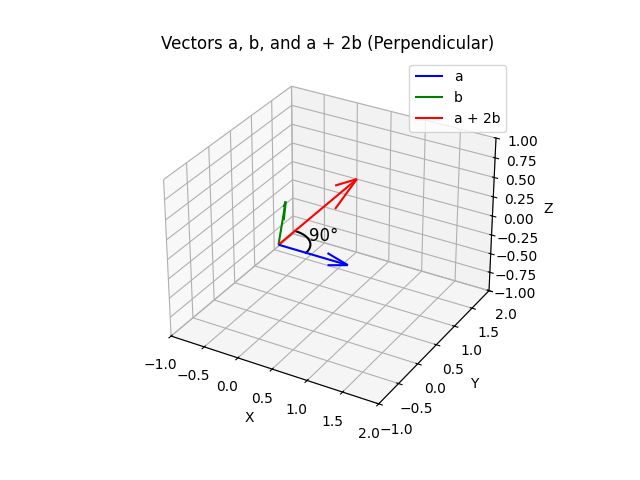
\includegraphics[width=0.6\columnwidth]{../figs/graph4.png}
\end{center}
\caption{}
\label{fig:Fig}
\end{figure}  
\end{frame}



\begin{frame}[fragile]
    \frametitle{Python Code}
    \begin{lstlisting}
# Plot origin
origin = np.zeros(3)

# Plot vectors
ax.quiver(*origin, *a, color='blue', label='a')
ax.quiver(*origin, *b, color='green', label='b')
ax.quiver(*origin, *a_plus_2b, color='red', label='a + 2b')

# ---- Add 90-degree arc ----
# Normalize vectors
a_unit = a / np.linalg.norm(a)
a2b_unit = a_plus_2b / np.linalg.norm(a_plus_2b)

# Create arc between a and a+2b
theta = np.linspace(0, np.pi / 2, 30)
arc_radius = 0.4
arc_points = np.array([arc_radius * (np.cos(t) * a_unit + np.sin(t) * a2b_unit) for t in theta])

\end{lstlisting}
\end{frame}

\begin{frame}[fragile]
    \frametitle{Python Code}

    \begin{lstlisting}
# Plot the arc
ax.plot(arc_points[:, 0], arc_points[:, 1], arc_points[:, 2], color='black')

# Label the angle
angle_label_pos = arc_radius * (np.cos(np.pi / 4) * a_unit + np.sin(np.pi / 4) * a2b_unit)
ax.text(*angle_label_pos, "90°", fontsize=12, color='black')

# Axis settings
ax.set_xlabel('X')
ax.set_ylabel('Y')
ax.set_zlabel('Z')
ax.set_xlim([-1, 2])
ax.set_ylim([-1, 2])
ax.set_zlim([-1, 1])
ax.legend()


    \end{lstlisting}
\end{frame}

\begin{frame}[fragile]
    \frametitle{Python Code}

    \begin{lstlisting}
# Save figure
plt.savefig("graph4.png")
print("Saved as graph4.png")

# Optional: Show the plot
# plt.show()





  \end{lstlisting}
\end{frame}

\begin{frame}[fragile]
\frametitle{C Code}
\begin{lstlisting}
include <stdio.h>
#include <math.h>

#define EPS 1e-6

// Compute dot product of two 2D vectors stored as 1×2 matrices
// a: array double a[2]; b: array double b[2]
double dot2(const double a[2], const double b[2]) {
    return a[0]*b[0] + a[1]*b[1];
}

// Solve the question using matrix-like vector operations
// returns 1 if (a + 2b) is perpendicular to a under the condition ||a + b|| == ||b||, else 0

    \end{lstlisting}

\end{frame}

\begin{frame}[fragile]
\frametitle{C Code}
\begin{lstlisting}
  int solve_matrix_vectors(double a0, double a1, double b0, double b1) {
    double a_vec[2] = { a0, a1 };
    double b_vec[2] = { b0, b1 };

    double ab_vec[2] = { a0 + b0, a1 + b1 };     // a + b
    double b_norm2 = dot2(b_vec, b_vec);         // ||b||^2
    double ab_norm2 = dot2(ab_vec, ab_vec);       // ||a + b||^2

    if (fabs(ab_norm2 - b_norm2) > EPS) {
        // Condition ||a + b|| == ||b|| fails
        return 0;
    }
\end{lstlisting}
\end{frame}
\begin{frame}[fragile]
\frametitle{C Code}
\begin{lstlisting}
 double a2b_vec[2] = { a0 + 2.0 * b0, a1 + 2.0 * b1 };  // a + 2b

    double dp = dot2(a_vec, a2b_vec);    // a · (a + 2b)

    if (fabs(dp) < EPS) {
        // Perpendicular
        return 1;
    } else {
        return 0;
    }
}

\end{lstlisting}
\end{frame}


\begin{frame}[fragile]
\frametitle{Python and C Code}

\begin{lstlisting}
import ctypes
import os

# locate shared library
_dir = os.path.dirname(__file__)
lib_path = os.path.join(_dir, "libmatrix_vectors.so")

lib = ctypes.CDLL(lib_path)

# declare the argument types and return type
lib.solve_matrix_vectors.argtypes = [
    ctypes.c_double,  # a0 (ax)
    ctypes.c_double,  # a1 (ay)
    ctypes.c_double,  # b0 (bx)
    ctypes.c_double   # b1 (by)
]
\end{lstlisting}

\end{frame}
\begin{frame}[fragile]
\frametitle{Python and C Code}

\begin{lstlisting}
lib.solve_matrix_vectors.restype = ctypes.c_int

def solve_matrix_vectors(a0, a1, b0, b1):
    """Wrapper function returning True / False."""
    res = lib.solve_matrix_vectors(ctypes.c_double(a0),
                                   ctypes.c_double(a1),
                                   ctypes.c_double(b0),
                                   ctypes.c_double(b1))
    return bool(res)

if __name__ == "__main__":
    # Examples
    a0, a1 = 2.0, 1.0
    b0, b1 = 1.0, 2.0

    if solve_matrix_vectors(a0, a1, b0, b1):
        print("(a + 2b) is perpendicular to a under the condition ||a + b|| = ||b||")
    else:
        print("Condition fails or not perpendicular.")
\end{lstlisting}

\end{frame}

 





\end{document}